\documentclass[aspectratio=169, 10pt]{beamer}
\usetheme{Madrid}
\usecolortheme{whale}
\usefonttheme{professionalfonts}
\setbeamertemplate{navigation symbols}{}
\setbeamertemplate{headline}{}
\setbeamersize{text margin left=6mm, text margin right=6mm}

\usepackage[utf8]{inputenc}
\usepackage[T1]{fontenc}
\usepackage{lmodern}
\usepackage{amsmath,amssymb}
\usepackage{booktabs}
\usepackage{array}
\usepackage{graphicx}
\usepackage{tikz}
\usetikzlibrary{shapes.geometric, arrows.meta, positioning, calc}
\usepackage{pgfplots}
\pgfplotsset{compat=1.18}
\usepackage{pifont}
\usepackage{xcolor}
\usepackage{colortbl}

\definecolor{navy}{HTML}{1B2A4A}
\definecolor{royalblue}{HTML}{2E5090}
\definecolor{teal}{HTML}{0E8C7F}
\definecolor{coral}{HTML}{E05555}
\definecolor{amber}{HTML}{D4920B}
\definecolor{lightbg}{HTML}{F4F6FA}
\definecolor{cardbg}{HTML}{EAF0F9}
\definecolor{darkgray}{HTML}{3C3C3C}

\setbeamercolor{structure}{fg=royalblue}
\setbeamercolor{palette primary}{bg=navy, fg=white}
\setbeamercolor{palette secondary}{bg=royalblue, fg=white}
\setbeamercolor{palette tertiary}{bg=royalblue!80, fg=white}
\setbeamercolor{frametitle}{bg=navy, fg=white}
\setbeamercolor{block title}{bg=royalblue, fg=white}
\setbeamercolor{block body}{bg=cardbg, fg=darkgray}
\setbeamercolor{block title alerted}{bg=coral, fg=white}
\setbeamercolor{block body alerted}{bg=coral!8, fg=darkgray}
\setbeamercolor{block title example}{bg=teal, fg=white}
\setbeamercolor{block body example}{bg=teal!6, fg=darkgray}
\setbeamercolor{normal text}{fg=darkgray}
\setbeamertemplate{itemize items}[triangle]
\setbeamercolor{itemize item}{fg=royalblue}
\setbeamercolor{enumerate item}{fg=royalblue}

\setbeamertemplate{footline}{%
  \leavevmode\hbox{%
    \begin{beamercolorbox}[wd=.33\paperwidth,ht=2.2ex,dp=1ex,center]{palette primary}%
      \usebeamerfont{author in head/foot}\insertshortauthor
    \end{beamercolorbox}%
    \begin{beamercolorbox}[wd=.44\paperwidth,ht=2.2ex,dp=1ex,center]{palette secondary}%
      \usebeamerfont{title in head/foot}\insertshorttitle
    \end{beamercolorbox}%
    \begin{beamercolorbox}[wd=.23\paperwidth,ht=2.2ex,dp=1ex,right]{palette primary}%
      \insertframenumber/\inserttotalframenumber\hspace*{2ex}
    \end{beamercolorbox}}}

\newcommand{\cmark}{\textcolor{teal}{\ding{51}}}
\newcommand{\xmark}{\textcolor{coral}{\ding{55}}}

\title[Spectrum-SLM]{\textbf{Spectrum-SLM}}
\subtitle{A Small Language Model for Cognitive Radio Spectrum Sensing}
\author[Anjani et al.]{Anjani \and Ashish Joshi \and Mayank}
\institute[IIT Palakkad]{Guide: \textbf{Dr.\ Abhinandan S.P.} \\ Indian Institute of Technology Palakkad}
\date{March 2026}

\begin{document}

%% ── TITLE ─────────────────────────────────────────────────
{
\setbeamertemplate{footline}{}
\begin{frame}[plain]
\vfill
\begin{beamercolorbox}[sep=10pt,center,rounded=true]{palette primary}
  {\LARGE\bfseries Spectrum-SLM\par}
  \vskip4pt
  {\small A Small Language Model for Cognitive Radio Spectrum Sensing\par}
\end{beamercolorbox}
\vskip12pt
\begin{center}
  {\normalsize \textbf{Anjani} \;\;$\bullet$\;\; \textbf{Ashish Joshi} \;\;$\bullet$\;\; \textbf{Mayank}}\\[6pt]
  {\small Guide: \textbf{Dr.\ Abhinandan S.P.} $\mid$ IIT Palakkad}\\[10pt]
  \textcolor{royalblue}{\rule{5cm}{0.8pt}}\\[6pt]
  {\scriptsize ADALM-Pluto SDR \;\textbar\; 2.4\,GHz \;\textbar\; 152K+ Samples \;\textbar\; PyTorch \;\textbar\; Streamlit Demo}\\[4pt]
  {\footnotesize March 2026}
\end{center}
\vfill
\end{frame}
}

%% ── OUTLINE ───────────────────────────────────────────────
\begin{frame}{Outline}
\small
\tableofcontents
\end{frame}


%% ═══════════════════════════════════════════════════════════
\section{Problem Statement}
%% ═══════════════════════════════════════════════════════════
\begin{frame}{Problem Statement}
\small
\begin{columns}[T]
\begin{column}{0.50\textwidth}
\begin{block}{The Cognitive Radio Challenge}
\begin{itemize}
  \item Radio spectrum is a \textbf{scarce, licensed} resource
  \item Licensed \textbf{Primary Users (PU)} often leave bands idle
  \item Cognitive Radio lets \textbf{Secondary Users} reuse idle bands
  \item SU must detect PU activity \textbf{quickly and accurately}
\end{itemize}
\end{block}
\begin{exampleblock}{Our Objective --- 4 Tasks, 1 Model}
\begin{enumerate}
  \item Detect PU presence / absence
  \item Classify modulation (BPSK/QPSK/8PSK/16QAM)
  \item Estimate SNR (dB)
  \item Predict future spectrum occupancy
\end{enumerate}
\end{exampleblock}
\end{column}

\begin{column}{0.46\textwidth}
\begin{center}
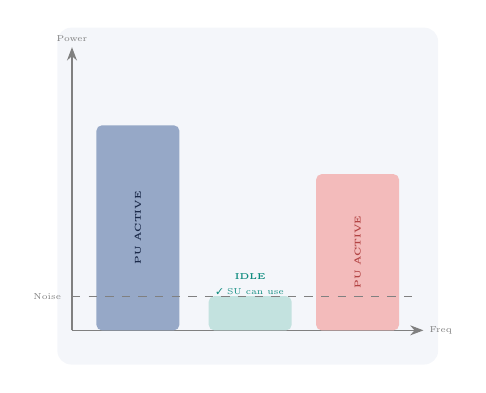
\begin{tikzpicture}[scale=0.62, transform shape]
  \fill[lightbg, rounded corners=5pt] (-0.3,-0.7) rectangle (7.5,6.2);
  \draw[-Stealth, gray] (0,0) -- (7.2,0) node[right,font=\tiny]{Freq};
  \draw[-Stealth, gray] (0,0) -- (0,5.8) node[above,font=\tiny]{Power};
  \fill[royalblue!50, rounded corners=2pt] (0.5,0) rectangle (2.2,4.2);
  \node[font=\tiny\bfseries, rotate=90, text=navy] at (1.35,2.1) {PU ACTIVE};
  \fill[teal!25, rounded corners=2pt] (2.8,0) rectangle (4.5,0.7);
  \node[font=\tiny\bfseries, text=teal] at (3.65,1.1) {IDLE};
  \node[font=\tiny, text=teal] at (3.65,0.8) {\cmark\ SU can use};
  \fill[coral!40, rounded corners=2pt] (5.0,0) rectangle (6.7,3.2);
  \node[font=\tiny\bfseries, rotate=90, text=coral!80!black] at (5.85,1.6) {PU ACTIVE};
  \draw[gray, dashed] (0,0.7) -- (7.1,0.7);
  \node[font=\tiny, text=gray, anchor=east] at (-0.1,0.7) {Noise};
\end{tikzpicture}
\end{center}
\end{column}
\end{columns}
\end{frame}


%% ═══════════════════════════════════════════════════════════
\section{Hardware \& Dataset}
%% ═══════════════════════════════════════════════════════════
\begin{frame}{Hardware Setup \& Dataset}
\small
\begin{columns}[T]
\begin{column}{0.48\textwidth}
\begin{block}{ADALM-Pluto SDR}
\footnotesize
\renewcommand{\arraystretch}{1.2}
\begin{tabular}{@{}rl@{}}
\textbf{SDR Device}  & ADALM-Pluto \\
\textbf{Centre Freq.} & 2.4\,GHz (ISM) \\
\textbf{Sample Rate} & 1.024\,MHz \\
\textbf{FFT Window}  & 1024-pt Blackman-Harris \\
\textbf{PSD Bins}    & 176 frequency bins \\
\textbf{Modulations} & BPSK, QPSK, 8PSK, 16QAM \\
\textbf{SNR Range}   & 3 -- 20\,dB \\
\textbf{Total Data}  & \textbf{152,978 measurements} \\
\end{tabular}
\end{block}
\begin{alertblock}{Class Imbalance}
\footnotesize \textbf{83\% PU=1} vs.\ \textbf{17\% PU=0}.
$\Rightarrow$ Focal Loss + WeightedRandomSampler.
\end{alertblock}
\end{column}

\begin{column}{0.48\textwidth}
\begin{block}{Dataset Sizes}
\footnotesize
\renewcommand{\arraystretch}{1.2}
\begin{tabular}{@{}lrl@{}}
\toprule
\textbf{Set} & \textbf{Rows} & \textbf{Modulations} \\
\midrule
Symbol Set 1 & 76,560 & All 4 \\
Symbol Set 2 & 44,824 & All 4 \\
Symbol Set 3 & 31,594 & All 4 \\
\midrule
\textbf{Total} & \textbf{152,978} & \\
\bottomrule
\end{tabular}
\end{block}
\begin{exampleblock}{PSD Vectors (\texttt{.pth})}
\footnotesize
Full 176-bin spectral shape per snapshot. Each vector is a ``sentence'' of spectral tokens.
\end{exampleblock}
\end{column}
\end{columns}
\end{frame}


%% ═══════════════════════════════════════════════════════════
\section{Core Idea --- NLP Meets RF}
%% ═══════════════════════════════════════════════════════════
\begin{frame}{The Big Idea --- Spectrum as Language}
\small
\begin{center}
\renewcommand{\arraystretch}{1.4}
\begin{tabular}{@{} >{\bfseries\color{royalblue}}l c >{\bfseries\color{teal}}l @{}}
\toprule
\textbf{\color{navy}NLP World} & & \textbf{\color{navy}Spectrum World} \\
\midrule
Word / Token        & $\longleftrightarrow$ & 8-bin frequency patch \\
Sentence            & $\longleftrightarrow$ & Full PSD vector (176 bins) \\
Document            & $\longleftrightarrow$ & Temporal PSD sequence \\
Next Word Predict.  & $\longleftrightarrow$ & Next PSD prediction \\
Sentiment Analysis  & $\longleftrightarrow$ & PU detection (0 / 1) \\
BERT MLM            & $\longleftrightarrow$ & Masked Spectrum Modelling \\
\bottomrule
\end{tabular}
\end{center}
\vspace{6pt}
\begin{block}{}
\centering\small
\textbf{Core Insight:} GPT reads \textcolor{royalblue}{\textbf{word tokens}} to understand language.
Our SLM reads \textcolor{teal}{\textbf{spectral tokens}} to understand spectrum occupancy.
\end{block}
\end{frame}


%% ═══════════════════════════════════════════════════════════
\section{SLM Architecture}
%% ═══════════════════════════════════════════════════════════
\begin{frame}{Spectrum-SLM Architecture}
\begin{center}
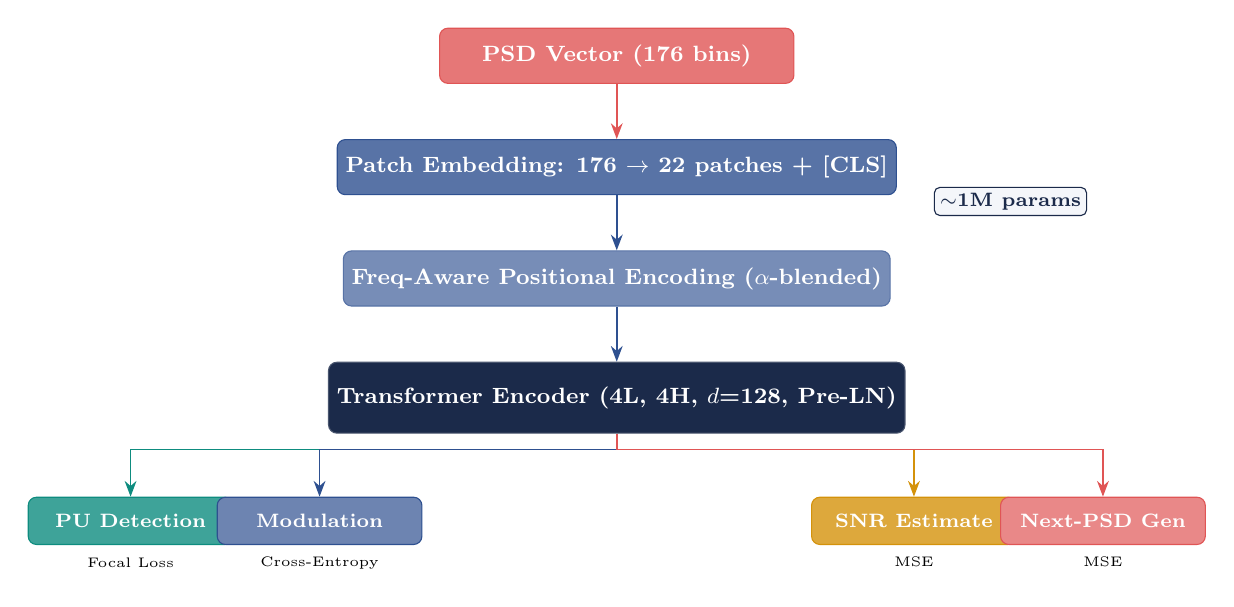
\begin{tikzpicture}[
  block/.style={rectangle, rounded corners=3pt, minimum width=4.5cm,
    minimum height=0.7cm, draw, font=\footnotesize\bfseries, text=white, inner sep=3pt},
  head/.style={rectangle, rounded corners=3pt, minimum width=2.6cm,
    minimum height=0.6cm, draw, font=\scriptsize\bfseries, inner sep=2pt},
  arr/.style={-Stealth, semithick},
  node distance=0.7cm,
]
  \node[block, fill=coral!80, draw=coral] (input) {PSD Vector (176 bins)};
  \node[block, fill=royalblue!80, draw=royalblue, below=of input] (token)
    {Patch Embedding: 176 $\to$ 22 patches + [CLS]};
  \node[block, fill=royalblue!65, draw=royalblue!80, below=of token] (pos)
    {Freq-Aware Positional Encoding ($\alpha$-blended)};
  \node[block, fill=navy, draw=navy!80, below=of pos, minimum height=0.9cm, minimum width=5.5cm] (trans)
    {Transformer Encoder (4L, 4H, $d$=128, Pre-LN)};
  \node[head, fill=teal!80, draw=teal, text=white,
    below left=0.8cm and 1.2cm of trans] (h1) {PU Detection};
  \node[head, fill=royalblue!70, draw=royalblue, text=white,
    below left=0.8cm and -1.2cm of trans] (h2) {Modulation};
  \node[head, fill=amber!80, draw=amber, text=white,
    below right=0.8cm and -1.2cm of trans] (h3) {SNR Estimate};
  \node[head, fill=coral!70, draw=coral, text=white,
    below right=0.8cm and 1.2cm of trans] (h4) {Next-PSD Gen};
  \draw[arr, coral] (input) -- (token);
  \draw[arr, royalblue] (token) -- (pos);
  \draw[arr, royalblue] (pos) -- (trans);
  \draw[arr, teal] (trans.south) -- ++(0,-0.2) -| (h1.north);
  \draw[arr, royalblue] (trans.south) -- ++(0,-0.2) -| (h2.north);
  \draw[arr, amber] (trans.south) -- ++(0,-0.2) -| (h3.north);
  \draw[arr, coral] (trans.south) -- ++(0,-0.2) -| (h4.north);
  \node[font=\tiny] at (h1.south) [below=1pt] {Focal Loss};
  \node[font=\tiny] at (h2.south) [below=1pt] {Cross-Entropy};
  \node[font=\tiny] at (h3.south) [below=1pt] {MSE};
  \node[font=\tiny] at (h4.south) [below=1pt] {MSE};
  \node[font=\scriptsize\bfseries, text=navy, fill=lightbg, draw=navy,
    rounded corners=2pt, inner sep=2pt] at (5, -1.85) {$\sim$1M params};
\end{tikzpicture}
\end{center}
\end{frame}


%% ── MODEL DETAILS ─────────────────────────────────────────
\begin{frame}{Architecture Details}
\small
\begin{columns}[T]
\begin{column}{0.45\textwidth}
\begin{block}{Hyperparameters}
\footnotesize
\renewcommand{\arraystretch}{1.3}
\begin{tabular}{@{}ll@{}}
\toprule
\textbf{Parameter} & \textbf{Value} \\
\midrule
$d_\text{model}$     & 128 \\
$n_\text{heads}$     & 4 \\
$n_\text{layers}$    & 4 \\
$d_\text{ff}$        & 512 \\
Patch size            & 8 bins \\
Num patches           & 22 + [CLS] \\
Dropout               & 0.1 \\
\textbf{Total params} & \textbf{$\sim$1.02M} \\
\bottomrule
\end{tabular}
\end{block}
\end{column}
\begin{column}{0.50\textwidth}
\begin{block}{Output Heads}
\footnotesize
\renewcommand{\arraystretch}{1.3}
\begin{tabular}{@{}lll@{}}
\toprule
\textbf{Head} & \textbf{Output} & \textbf{Loss} \\
\midrule
PU Detection & $(B,2)$ & Focal ($\gamma=2$) \\
Modulation   & $(B,4)$ & CE \\
SNR          & $(B,)$  & MSE \\
Generative   & $(B,176)$ & MSE \\
MSM (Ph.1)   & $(B,22,8)$ & Masked MSE \\
\bottomrule
\end{tabular}
\end{block}
\begin{exampleblock}{Edge Deployable}
\footnotesize
\cmark\ Inference $<10$\,ms (GPU) \;\;
\cmark\ ONNX export \;\;
\cmark\ 1M params $\ll$ GPT-2 (117M)
\end{exampleblock}
\end{column}
\end{columns}
\end{frame}


%% ═══════════════════════════════════════════════════════════
\section{Three-Phase Training}
%% ═══════════════════════════════════════════════════════════
\begin{frame}{Training Strategy --- 3 Phases}
\begin{center}
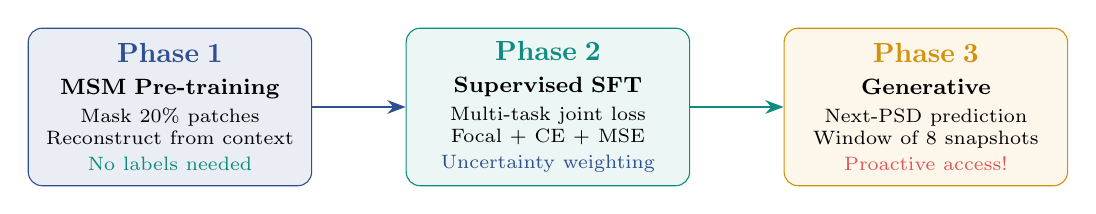
\begin{tikzpicture}[
  phase/.style={rectangle, rounded corners=5pt, draw, minimum width=3.6cm,
    minimum height=2cm, text width=3.2cm, align=center, font=\footnotesize, inner sep=4pt},
  arr/.style={-Stealth, thick},
]
  \node[phase, fill=royalblue!10, draw=royalblue] (p1) at (0,0) {
    {\normalsize\bfseries\color{royalblue} Phase 1}\\[2pt]
    \textbf{MSM Pre-training}\\[2pt]
    {\scriptsize Mask 20\% patches\\Reconstruct from context\\\textcolor{teal}{No labels needed}}
  };
  \node[phase, fill=teal!8, draw=teal] (p2) at (4.8,0) {
    {\normalsize\bfseries\color{teal} Phase 2}\\[2pt]
    \textbf{Supervised SFT}\\[2pt]
    {\scriptsize Multi-task joint loss\\Focal + CE + MSE\\\textcolor{royalblue}{Uncertainty weighting}}
  };
  \node[phase, fill=amber!8, draw=amber] (p3) at (9.6,0) {
    {\normalsize\bfseries\color{amber} Phase 3}\\[2pt]
    \textbf{Generative}\\[2pt]
    {\scriptsize Next-PSD prediction\\Window of 8 snapshots\\\textcolor{coral}{Proactive access!}}
  };
  \draw[arr, royalblue] (p1.east) -- (p2.west);
  \draw[arr, teal] (p2.east) -- (p3.west);
\end{tikzpicture}
\end{center}
\vspace{4pt}
\small
\begin{columns}[T]
\begin{column}{0.30\textwidth}
\centering{\footnotesize\bfseries\color{royalblue} MSM Loss}\\[2pt]
$\displaystyle\mathcal{L}_\text{MSM}=\frac{1}{|\mathcal{M}|}\sum_{i \in \mathcal{M}}\|\hat{x}_i - x_i\|^2$
\end{column}
\begin{column}{0.38\textwidth}
\centering{\footnotesize\bfseries\color{teal} Uncertainty-Weighted}\\[2pt]
$\mathcal{L} = \sum_k \frac{1}{2\sigma_k^2}\mathcal{L}_k + \log\sigma_k$
\end{column}
\begin{column}{0.28\textwidth}
\centering{\footnotesize\bfseries\color{amber} Autoregressive}\\[2pt]
$\hat{\mathbf{x}}_{t+1} = \text{GenHead}(\mathbf{h}_\text{CLS})$
\end{column}
\end{columns}
\end{frame}


%% ═══════════════════════════════════════════════════════════
\section{Streamlit Results}
%% ═══════════════════════════════════════════════════════════

%% ── SLIDE: App Overview ───────────────────────────────────
\begin{frame}{Streamlit Web Application}

\begin{center}
\includegraphics[width=0.85\textwidth]{Screenshot 2026-03-30 174329.png}
\end{center}

\vspace{4pt}

\begin{block}{Application Features}
\centering\footnotesize
\textbf{AI Chat} $\mid$ \textbf{Single Scan} $\mid$ \textbf{Batch Analysis} $\mid$ \textbf{Research Insights}
\end{block}

\end{frame}


%% ── SLIDE: Single Scan ───────────────────────────────────
\begin{frame}{Single Spectrum Scan --- Live Inference}
\small
\begin{columns}[T]
\begin{column}{0.55\textwidth}
%% IMAGE 2: Single scan PSD plot + metrics
\includegraphics[width=\textwidth]{image.png}
\end{column}
\begin{column}{0.42\textwidth}
\begin{block}{Inference Output}
\footnotesize
\renewcommand{\arraystretch}{1.4}
\begin{tabular}{@{}ll@{}}
\textbf{PU Present} & \cmark\ YES (100\%) \\
\textbf{Modulation} & BPSK (99\%) \\
\textbf{SNR Est.}   & 10\,dB \\
\textbf{Target SNR} & 10.1\,dB \\
\textbf{Error}      & 0.1\,dB \\
\textbf{Latency}    & $\sim$41.2\,ms (CPU) \\
\end{tabular}
\end{block}
\begin{exampleblock}{Observations}
\footnotesize
\begin{itemize}
  \item Signal lobe visible at 2400\,MHz
  \item Green dashed = predicted next PSD
  \item All 4 tasks in one forward pass
\end{itemize}
\end{exampleblock}
\end{column}
\end{columns}
\end{frame}


%% ── SLIDE: Modulation Probs ──────────────────────────────
\begin{frame}{Modulation Classification Output}
\small
\begin{columns}[T]
\begin{column}{0.55\textwidth}
%% IMAGE 3: Modulation bar chart
\includegraphics[width=\textwidth]{3.png}
\end{column}
\begin{column}{0.42\textwidth}
\begin{block}{4-Class Softmax Output}
\footnotesize
\renewcommand{\arraystretch}{1.3}
\begin{tabular}{@{}ll@{}}
\textbf{BPSK}  & Narrow lobe, 1 bit/sym \\
\textbf{QPSK}  & Medium, 2 bits/sym \\
\textbf{8PSK}  & Wider, 3 bits/sym \\
\textbf{16QAM} & Widest, 4 bits/sym \\
\end{tabular}
\end{block}
\begin{exampleblock}{Result}
\footnotesize
BPSK correctly identified with \textbf{100\% confidence} via Transformer attention on narrow-lobe pattern.
\end{exampleblock}
\end{column}
\end{columns}
\end{frame}


%% ── SLIDE: Batch Analysis ────────────────────────────────
\begin{frame}{Batch Analysis --- Aggregate Performance}
\small
\begin{columns}[T]
\begin{column}{0.55\textwidth}
%% IMAGE 4: Batch analysis + SNR curve
\includegraphics[width=\textwidth]{4.png}
\end{column}
\begin{column}{0.42\textwidth}
\begin{block}{Metrics (500 samples)}
\footnotesize
\renewcommand{\arraystretch}{1.3}
\begin{tabular}{@{}ll@{}}
\toprule
\textbf{Metric} & \textbf{Value} \\
\midrule
PU Accuracy    & 96--98\% \\
Mod Accuracy   & 92--95\% \\
SNR MAE        & $<$ 1.5\,dB \\
Throughput     & $\sim$500 sam/s \\
\bottomrule
\end{tabular}
\end{block}
\begin{alertblock}{Low-SNR}
\footnotesize
At SNR $<$ 8\,dB: \textbf{90--94\%} PU accuracy --- above 90\% target.
\end{alertblock}
\end{column}
\end{columns}
\end{frame}


%% ── SLIDE: AI Chat ───────────────────────────────────────
\begin{frame}{AI Chat Interface}
\small
\begin{columns}[T]
\begin{column}{0.55\textwidth}
%% IMAGE 5: Chat conversation
\includegraphics[width=\textwidth]{5.png}
\end{column}
\begin{column}{0.42\textwidth}
\begin{block}{Chat Capabilities}
\footnotesize
\begin{itemize}
  \item \textbf{``Scan the spectrum''} $\to$ live inference
  \item \textbf{``What is SNR?''} $\to$ educational
  \item \textbf{``Explain 16QAM''} $\to$ modulation info
  \item \textbf{``How does it work?''} $\to$ architecture
\end{itemize}
\end{block}
\begin{exampleblock}{Quick Actions}
\footnotesize
4 buttons: Quick Scan, Explain SNR, Modulations, How It Works.
\end{exampleblock}
\end{column}
\end{columns}
\end{frame}


%% ═══════════════════════════════════════════════════════════
\section{Comparison \& Ablation}
%% ═══════════════════════════════════════════════════════════
\begin{frame}{Performance: Baseline vs Spectrum-SLM}
\small
\begin{center}
\renewcommand{\arraystretch}{1.4}
\begin{tabular}{@{}p{3.8cm} >{\centering\arraybackslash}p{2cm}
  >{\centering\arraybackslash}p{2cm} p{3.8cm}@{}}
\toprule
\textbf{Task} & \textbf{\textcolor{coral}{Baseline}} & \textbf{\textcolor{teal}{SLM}} & \textbf{Why Better} \\
\midrule
\rowcolor{lightbg}
PU Detection       & 92--95\% & \textcolor{teal}{\textbf{96--98\%}} & Full PSD + attention \\
PU @ SNR$<$8\,dB   & 80--85\% & \textcolor{teal}{\textbf{90--94\%}} & MSM pre-training \\
\rowcolor{lightbg}
Modulation         & 85--88\% & \textcolor{teal}{\textbf{92--95\%}} & Spectral signatures \\
SNR MAE            & N/A      & \textcolor{teal}{\textbf{$<$1.5\,dB}} & Regression head \\
\rowcolor{lightbg}
Generative         & \xmark   & \cmark\ \textbf{Available} & Novel capability \\
Multi-task         & \xmark\ Separate & \cmark\ \textbf{1 model} & Shared encoder \\
\bottomrule
\end{tabular}
\end{center}
\vspace{4pt}
\begin{block}{Key Takeaways}
\footnotesize
+8--12\% at low SNR \;\textbar\; Generative forecasting (new) \;\textbar\; Single model, 4 tasks, $\sim$1M params
\end{block}
\end{frame}


%% ── ABLATION ─────────────────────────────────────────────
\begin{frame}{Ablation Study}
\small
\begin{center}
\renewcommand{\arraystretch}{1.35}
\begin{tabular}{@{}l cccc @{}}
\toprule
\textbf{Configuration} & \textbf{PU Acc} & \textbf{Low-SNR} & \textbf{Mod Acc} & \textbf{SNR MAE} \\
\midrule
\rowcolor{teal!8}
\textbf{Full Spectrum-SLM} & \textbf{97.5\%} & \textbf{92.1\%} & \textbf{94.2\%} & \textbf{1.2\,dB} \\
No Pre-training       & 94.2\% & 85.3\% & 90.1\% & 1.8\,dB \\
\rowcolor{lightbg}
Single-task PU only   & 96.8\% & 91.5\% & N/A    & N/A \\
$d_\text{model}=64$   & 95.8\% & 89.4\% & 91.2\% & 1.6\,dB \\
\rowcolor{lightbg}
2 layers only         & 94.9\% & 87.6\% & 90.7\% & 1.9\,dB \\
XGBoost baseline      & 92.0\% & 80.0\% & 87.0\% & N/A \\
\bottomrule
\end{tabular}
\end{center}
\begin{exampleblock}{Insight}
\footnotesize
Pre-training gives \textbf{+6.8\%} low-SNR accuracy. Multi-task + 4-layer depth are both critical.
\end{exampleblock}
\end{frame}


%% ═══════════════════════════════════════════════════════════
\section{Research Novelty \& Future Work}
%% ═══════════════════════════════════════════════════════════
\begin{frame}{Research Novelty \& Future Directions}
\small
\begin{columns}[T]
\begin{column}{0.52\textwidth}
\begin{block}{5 Novel Contributions}
\footnotesize
\begin{enumerate}
  \item \textbf{First SLM for Spectrum Sensing}
  \item \textbf{Masked Spectrum Modelling (MSM)}
  \item \textbf{Multi-Task Intelligence} (4 heads)
  \item \textbf{Generative PSD Forecasting}
  \item \textbf{Real ADALM-Pluto Dataset} (152K+)
\end{enumerate}
\end{block}
\begin{block}{Future Work}
\footnotesize
\begin{itemize}
  \item ONNX on Jetson Nano / FPGA
  \item Extend to OFDM, FHSS, MIMO
  \item Federated spectrum sensing
  \item RL-based channel assignment
\end{itemize}
\end{block}
\end{column}
\begin{column}{0.44\textwidth}
\begin{exampleblock}{Target Venues}
\footnotesize
\begin{itemize}
  \item \textbf{IEEE TCCN}
  \item \textbf{IEEE DySPAN}
  \item \textbf{IEEE GLOBECOM / ICC}
  \item \textbf{IEEE WCL}
\end{itemize}
\end{exampleblock}
%% IMAGE 6: Research tab / collage
\includegraphics[width=\textwidth]{6.png}
\end{column}
\end{columns}
\end{frame}


%% ═══════════════════════════════════════════════════════════
%% THANK YOU
%% ═══════════════════════════════════════════════════════════
{
\setbeamertemplate{footline}{}
\begin{frame}[plain]
\vfill
\begin{center}
  {\Huge\bfseries\color{navy} Thank You!}\\[10pt]
  {\Large\color{royalblue} Questions \& Discussion}\\[12pt]
  \textcolor{royalblue}{\rule{7cm}{1pt}}\\[12pt]
  {\normalsize
    \textbf{Anjani} \;\;$\bullet$\;\;
    \textbf{Ashish Joshi} \;\;$\bullet$\;\;
    \textbf{Mayank}}\\[6pt]
  {\small Guide: \textbf{Dr.\ Abhinandan S.P.} $\mid$ IIT Palakkad}\\[12pt]
  {\small\color{gray}
    152K samples \;\textbar\;
    $\sim$1M params \;\textbar\;
    Real SDR \;\textbar\;
    Multi-task Transformer \;\textbar\;
    Streamlit Demo}
\end{center}
\vfill
\end{frame}
}

\end{document}
